\chapter{Implementierung}
Das Verfahren wurde im Rahmen des Projektes in einen OpenGl C++ Programm umgesetzt.
Um die 2D Schatten zu implementieren müssen zwingend Framebuffer benutzt werden.
Ohne Verwendung von Framebuffern können die entsprechenden Texturen nicht erstellt werden die zu Berechnung der Schatten benötigt werden. 
\begin{figure}[h]
	\centering
	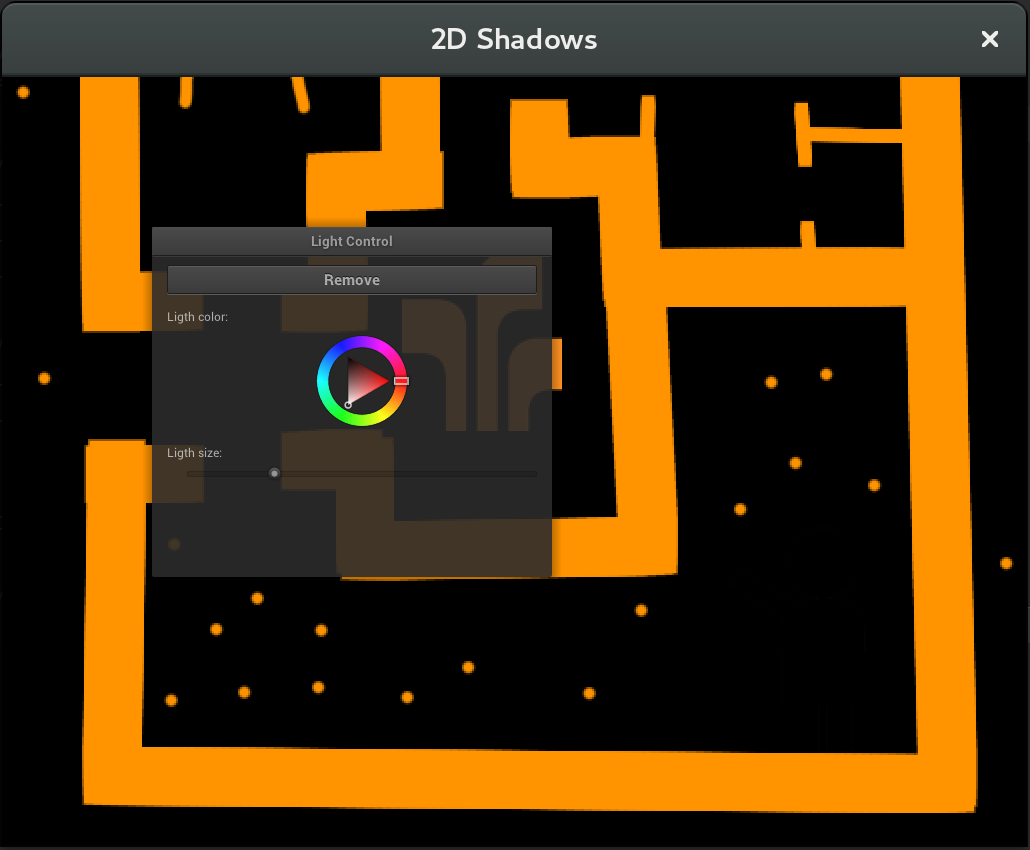
\includegraphics[scale=0.25]{images/Bildschirmfoto_1.png}
	\caption{Programm beim nach dem Start.}
	\label{p_1}
\end{figure}

Die Schritte die hier beschrieben werden müssen für jedes neue Licht durchgeführt werden.
\newpage
\section{Oclussionmap}

Für die Oclussionmap wird eine Textur angelegt die der Größe des Lichtes entspricht.
\begin{lstlisting}
// The texture we're going to render to
GLuint oclusion_texture;
glGenTextures(1, &oclusion_texture);

// "Bind" the newly created texture : 
// all future texture functions will modify this texture
glBindTexture(GL_TEXTURE_2D, oclusion_texture);

// Give an empty image to OpenGL ( the last "0" )
glTexImage2D(GL_TEXTURE_2D, 0,GL_RGBA8,
		 ligthsize, ligthsize, 0,
		 GL_RGBA, GL_UNSIGNED_BYTE, 0);
\end{lstlisting}

Diese wird nun an ein FBO gebunden.
\begin{lstlisting}
// Set "oclusion_texture" as our colour attachement #0
glFramebufferTexture(GL_FRAMEBUFFER, GL_COLOR_ATTACHMENT0, 
					 oclusion_texture, 0);
\end{lstlisting}

Jetzt werden die Occluder mit der entsprechen Transformierung gerendert um den vom Licht abgedeckten Bereich zu erfassen.
\begin{lstlisting}
auto mvp = glm::mat4{1};
auto ligthsize_half = (ligthsize/2.f);
mvp = glm::ortho(0.f, float(ligthsize), 0.f, float(ligthsize));
mvp *= glm::translate(glm::mat4{1},
			glm::vec3(-pos.x+ligthsize_half,-pos.y+ligthsize_half,0));
render_ocluders(mvp);
\end{lstlisting}

Dabei wird kein Spezieller Shader benutzt es ist nur wichtig das die Alphakanal Informationen vorhanden sind.

\section{Shadowmap}
Um die 1D Shadowmap zu erzeugen wird ein neuer Framebuffer mit einer Textur erzeugt die nur 1 Pixelhoch ist.
\begin{lstlisting}
GLuint shadow1D_texture;
glGenTextures(1, &shadow1D_texture);

glBindTexture(GL_TEXTURE_2D, shadow1D_texture);

// Give an empty image to OpenGL ( the last "0" )
glTexImage2D(GL_TEXTURE_2D, 0,GL_RGBA8, ligthsize,1,
		 0,GL_RGBA, GL_UNSIGNED_BYTE, 0);

glTexParameteri(GL_TEXTURE_2D, GL_TEXTURE_MAG_FILTER, GL_LINEAR);
glTexParameteri(GL_TEXTURE_2D, GL_TEXTURE_MIN_FILTER, GL_LINEAR);
//set to repeat so we can oversample the circle
glTexParameteri(GL_TEXTURE_2D, GL_TEXTURE_WRAP_S, GL_REPEAT); 
glTexParameteri(GL_TEXTURE_2D, GL_TEXTURE_WRAP_T, GL_REPEAT);


glFramebufferTexture(GL_FRAMEBUFFER, GL_COLOR_ATTACHMENT0,
					 shadow1D_texture, 0);
\end{lstlisting}

Jetzt muss nur noch der Viewport angepasst werden. Der Viewport wird auf die Breite des Lichtes gesetzt so das auf der X-Achse Parallelisiert einen Raycast auf der Occludertextur ausführen kann.

\begin{lstlisting}
glBindFramebuffer(GL_FRAMEBUFFER,shadow1D_fbo);
glViewport(0,0,ligthsize,1);
glClearColor(0.f,0.f,0.f,0.f);
glClear(GL_COLOR_BUFFER_BIT);

_shadow_mapper_shader->use_shader();
GLint id = _shadow_mapper_shader->getUniform("light_resolution");
glUniform2f(id,ligthsize,ligthsize);
glBindTexture(GL_TEXTURE_2D, oclusion_texture);


glBindVertexArray(quad_VertexArrayID);
glDrawArrays(GL_TRIANGLES,0,6);
\end{lstlisting}

\paragraph{Shader}
Der Shader\ref{shadow_shader} bekommt die Informationen wie groß die Occlusiontextur ist.
Da dieser Shader auf einem Mesh ausgeführt wird der nur einen einen Pixel hoch ist, wird jeder Punkt auf der Occlusiontextur exakt nur einmal gesampelt und die Tiefen Information in der 1D Textur als Grauwert gespeichert.

Der Shader basiert auf dem Shader von Matt DesLauriers \footnote{\url{https://gist.github.com/mattdesl/5286905\#file-shadowmap-frag}}
Der Shader wurde auf OpenGL 3.3 Modernisiert und PI etwas exakter gewählt.
\begin{lstlisting}[caption=Shadowmaper Shader,label=shadow_shader]
#version 330

#define PI 3.14159265359
in vec2 var_uv;

uniform sampler2D ocluder_texture;
uniform vec2 light_resolution;


//alpha threshold for our occlusion map
const float ALPHA_THRESHOLD = 0.75;

out vec4 out_color;

void main(){
float distance = 1.0;

for (float y=0.0; y<light_resolution.y; y+=1.0) {
//rectangular to polar filter
vec2 norm = vec2(var_uv.s, y/light_resolution.y) * 2.0 - 1.0;
float theta = PI*1.5 + norm.x * PI;
float r = (1.0 + norm.y) * 0.5;

//Coordinat which we will sample from occlude map
vec2 coord = vec2(-r * sin(theta), -r * cos(theta))/2.0 + 0.5;

//sample the occlusion map
vec4 data = texture2D(ocluder_texture, coord);

//the current distance is how far from the top we've come
float dst = y/light_resolution.y;

//if we've hit an opaque fragment (occluder), then get new distance
//if the new distance is below the current, then we'll use that for our ray
float caster = data.a;
if(isnan(caster)) caster = 1;

if (caster > ALPHA_THRESHOLD) {
distance = min(distance, dst);
}
}
out_color=vec4(vec3(distance), 1.0);
}
\end{lstlisting}

Abschließend wird die 1D Textur mit noch ein paar weiteren Informationen in einem \textit{Vector} abgelegt um später grendert zu werden, zum Beispiel Position Farbe und Größe.

\begin{lstlisting}
auto pic = add_image(ligthsize,ligthsize,false);

_ligth_images.emplace_back(std::get<0>(pic),std::get<1>(pic)
							,oclusion_texture,shadow1D_texture
							,glm::vec3{pos.x-(ligthsize/2.f)
							,pos.y-(ligthsize/2.f),0}
							,color,glm::vec2(size,size));
\end{lstlisting}

\section{Finales Rendering}
Beim Rendern der Schatten wird letztendlich nur noch die Distanz Informationen aus der 1D Textur gelesen und als Licht mit einem Falloff grendert. Für die bessere Optik wurde noch ein Gausfilter, in der stärke abhängig von der Entfernung zur Quelle, angewendet.

Der Shader basiert auf dem Shader von Matt DesLauriers \footnote{\url{https://gist.github.com/mattdesl/5286905\#file-shadowrender-frag}}
Der Shader wurde auf OpenGL 3.3 Modernisiert und PI etwas exakter gewählt.
Um bessere Kontrolle über die Farbe zu haben wurde das Vertex Colorattribut durch ein Uniform ersetzt. Zusätzlich wurden noch zwei Uniform variableren hinzugefügt um Kontrolle über den Falloff und Gaus-Blur zu haben.  
 \begin{lstlisting}[caption=Shadow Render Shader,label=shadow_render_shader]
#version 330

#define PI 3.14159265359

//inputs from vertex shader
in vec2 var_uv;

//uniform values
uniform sampler2D shadow_map_texture;
uniform vec2 light_resolution;
uniform vec4 Color;

//variable to signal if this light is selected 
//and how much blur it should have
uniform float selected;
uniform float blur_factor;


out vec4 out_color;

//sample from the 1D distance map
float sample(float coord, float r) {
return step(r, texture(shadow_map_texture, vec2(coord,0)).r);
}

void main(void) {
//rectangular to polar
vec2 norm = var_uv.st * 2.0 - 1.0;
float theta = atan(norm.y, norm.x);
float r = length(norm);
float coord = 1-(theta + PI) / (2.0*PI);

//the tex coord to sample our 1D lookup texture
//always 0.0 on y axis
vec2 tc = vec2(coord, 0.0);

//the center tex coord, which gives us hard shadows
float center = sample(coord, r);

//we multiply the blur amount by our distance from center
//this leads to more blurriness as the shadow "fades away"
float blur = (1./light_resolution.x) * smoothstep(0., 1., r);

//now we use a simple gaussian blur
float sum = 0.0;

sum += sample(coord - 4.0*blur, r) * 0.05;
sum += sample(coord - 3.0*blur, r) * 0.09;
sum += sample(coord - 2.0*blur, r) * 0.12;
sum += sample(coord - 1.0*blur, r) * 0.15;

sum += center * 0.16;

sum += sample(coord + 1.0*blur, r) * 0.15;
sum += sample(coord + 2.0*blur, r) * 0.12;
sum += sample(coord + 3.0*blur, r) * 0.09;
sum += sample(coord + 4.0*blur, r) * 0.05;

//sum of 1.0 -> in light, 0.0 -> in shadow

sum = (1-blur_factor)*sum + (blur_factor)*center;

//multiply the summed amount by our distance, which gives us a radial falloff
//then multiply by (light) color
out_color = Color * vec4(vec3(1.0)
						,sum * ((1-selected)*smoothstep(1.0, 0.0, r)+(selected)));
}
 \end{lstlisting}